\documentclass[sigconf,review,anonymous=false]{acmart} % review and anonymous=false for easier review, change for submission

% --- Core ACM Packages ---
\usepackage{booktabs} % For formal tables
\usepackage{graphicx} % For figures
\usepackage{amsmath}  % For math
\usepackage{amsfonts} % For math fonts
\usepackage{xcolor}   % For colors, if needed
\usepackage{colortbl} % For colored table cells, if needed
\usepackage{multirow} % For multi-row cells in tables
\usepackage{enumitem} % For customized lists
\usepackage{balance}  % To balance columns on the last page
\usepackage{hyperref} % For hyperlinks, load last usually
\hypersetup{
    colorlinks=true,
    linkcolor=blue,
    filecolor=magenta,
    urlcolor=cyan,
    citecolor=blue,
    pdftitle={Artificial Constitutionalism: A Self-Synthesizing Prompt Governance Compiler (ACGS-PGP) Framework for Advanced AI Systems},
    pdfpagemode=FullScreen,
    }

% --- Algorithm Package ---
\usepackage[ruled,vlined,linesnumbered]{algorithm2e}
\SetKwComment{Comment}{$\triangleright$\ }{}
\SetKwInOut{Input}{Input}
\SetKwInOut{Output}{Output}
\SetKwFunction{InterpretAC}{InterpretAC}
\SetKwFunction{GenerateBaselineRules}{GenerateBaselineRules}
\SetKwFunction{LoadExistingRules}{LoadExistingRules}
\SetKwFunction{PushToPGC}{PushToPGC}
\SetKwFunction{WaitForEvent}{WaitForEvent}
\SetKwFunction{IdentifyRulesFromFeedback}{IdentifyRulesFromFeedback}
\SetKwFunction{AdaptRule}{AdaptRule}
\SetKwFunction{AddToBuffer}{AddToBuffer}
\SetKwFunction{MapContextToAC}{MapContextToACPrinciples}
\SetKwFunction{UpdateInterpretation}{UpdateInterpretation}
\SetKwFunction{IdentifyImpactedRules}{IdentifyImpactedRules}
\SetKwFunction{ResynthesizeRule}{ResynthesizeRule}
\SetKwFunction{IdentifyNewRuleNeeds}{IdentifyNewRuleNeeds}
\SetKwFunction{SynthesizeNewRule}{SynthesizeNewRule}
\SetKwFunction{ProcessHumanDirective}{ProcessHumanDirective}
\SetKwFunction{SelectRulesForProactiveReview}{SelectRulesForProactiveReview}
\SetKwFunction{IsEmpty}{IsEmpty}
\SetKwFunction{ValidateRuleCandidates}{ValidateRuleCandidates}
\SetKwFunction{RequestHumanApprovalIfNeeded}{RequestHumanApprovalIfNeeded}
\SetKwFunction{UpdateOperationalRuleSet}{UpdateOperationalRuleSet}
\SetKwFunction{PGPSignRuleSet}{PGPSignRuleSet}
\SetKwFunction{LogGSAction}{LogGSAction}
\SetKwFunction{ClearBuffer}{ClearBuffer}


% --- Copyright Information (Update as per conference) ---
\copyrightyear{2025}
\acmYear{2025}
\setcopyright{acmlicensed} % Or rightsretained, usgov, etc.
\acmConference[FAccT '25]{Conference on Fairness, Accountability, and Transparency}{Month Day--Day, 2025}{City, Country}
\acmBooktitle{Conference on Fairness, Accountability, and Transparency (FAccT '25), Month Day--Day, 2025, City, Country}
\acmPrice{15.00}
\acmDOI{10.1145/XXXXXXX.XXXXXXX}
\acmISBN{978-X-XXXX-XXXX-X/YY/MM}


\begin{document}

% --- Title, Author, Affiliation ---
\title{Artificial Constitutionalism: A Self-Synthesizing Prompt Governance Compiler (ACGS-PGP) Framework for Advanced AI Systems}

\author{Martin Honglin Lyu}
\affiliation{%
  \institution{Soln AI}
  \city{Toronto}
  \state{Ontario}
  \country{Canada}
}
\email{martin@soln.ai}
\orcid{0000-0000-0000-0000} % Replace with actual ORCID

\renewcommand{\shortauthors}{Martin Honglin Lyu} % For running headers

% --- Abstract and CCS Concepts ---
\begin{abstract} % Max 250 words
The rapid proliferation and increasing autonomy of advanced Artificial Intelligence (AI) systems, particularly Large Language Model (LLM) agents, present profound governance challenges that outpace traditional regulatory and ethical oversight mechanisms. Existing approaches often lack the dynamism, verifiability, and embeddedness required to manage risks such as factual inaccuracies, opacity, data misuse, malicious exploitation, and bias. This paper introduces the Artificial Constitutionalism: Self-Synthesizing Prompt Governance Compiler (ACGS-PGP) framework, a novel, multi-layered architecture designed to embed dynamic, principled, and verifiable governance directly within AI systems. The framework's core components include: (1) an Artificial Constitution (AC), a foundational layer of adaptable normative principles; (2) a Self-Synthesizing (GS) Engine, an adaptive AI-driven mechanism that interprets the AC to generate context-specific operational governance rules; and (3) a Prompt Governance Compiler (PGC) with PGP Assurance, an enforcement layer that translates these rules into verifiable runtime constraints on AI behavior, ensuring policy integrity. By integrating high-level ethical and legal principles with an AI's operational logic, the ACGS-PGP framework aims to foster AI systems inherently aligned with human values, capable of dynamic adaptation, and subject to continuous, verifiable compliance. This research outlines the framework's design methodology, architecture, operational dynamics, conceptual validation through use cases, potential benefits, inherent challenges, and a research agenda, positioning it as a significant step towards trustworthy and accountable AI.
\end{abstract}

\begin{CCSXML}
<ccs2012>
   <concept>
       <concept_id>10003456.10003457.10003490.10003491</concept_id>
       <concept_desc>Social and professional topics~DESKTOP PUBLISHING</concept_desc>
       <concept_significance>500</concept_significance>
       </concept>
   <concept>
       <concept_id>10010147.10010178.10010179.10010182</concept_id>
       <concept_desc>Computing methodologies~Natural language generation</concept_desc>
       <concept_significance>500</concept_significance>
       </concept>
   <concept>
       <concept_id>10010147.10010178.10010224.10010245</concept_id>
       <concept_desc>Computing methodologies~Agent / discrete models</concept_desc>
       <concept_significance>500</concept_significance>
       </concept>
   <concept>
       <concept_id>10002978.10003006.10003017</concept_id>
       <concept_desc>Security and privacy~Formal methods</concept_desc>
       <concept_significance>300</concept_significance>
       </concept>
   <concept>
       <concept_id>10003456.10003462.10003487</concept_id>
       <concept_desc>Social and professional topics~Command and control systems</concept_desc>
       <concept_significance>300</concept_significance>
       </concept>
 </ccs2012>
\end{CCSXML}

\ccsdesc[500]{Social and professional topics~DESKTOP PUBLISHING}
\ccsdesc[500]{Computing methodologies~Natural language generation}
\ccsdesc[500]{Computing methodologies~Agent / discrete models}
\ccsdesc[300]{Security and privacy~Formal methods}
\ccsdesc[300]{Social and professional topics~Command and control systems}

\keywords{Artificial Intelligence Governance, LLM Agents, Artificial Constitutionalism, Self-Synthesizing Systems, Prompt Engineering, Formal Verification, AI Ethics, AI Safety, Compliance by Design}

\maketitle

% --- Main Body Sections ---
\section{Introduction}
Artificial intelligence (AI), particularly its generative forms like Large Language Models (LLMs), has rapidly advanced, becoming integral to diverse sectors. The increasing autonomy of LLM-based agentic systems to manage complex tasks and interact dynamically reached an inflection point in late 2022 with the widespread availability of consumer-facing generative AI~\cite{WorldBankAIGov24, LiMAST25}. The increasing autonomy of these AI agents allows them to plan, execute actions, and utilize external tools, significantly expanding their utility but also introducing novel and complex risks~\cite{AWSBedrockAgents}.

However, this integration brings significant risks. Five primary categories are broadly recognized [e.g., \cite{FPFGenAIGov24}]: factual inaccuracies, lack of transparency in operations~\cite{EuroParlAlgoTransparency19}, inappropriate use of personal data, malicious exploitation, and biased or discriminatory output~\cite{WorldBankAIGov24}. These risks are amplified by the "opacity of algorithmic systems"~\cite{EuroParlAlgoTransparency19} and the potential for AI to perpetuate societal biases~\cite{WorldBankAIGov24}. The increasing autonomy of LLM agents introduces new safety risks, including security vulnerabilities and unintended harmful actions~\cite{WangAgentSpec25}. This escalating capability and autonomy enlarge the attack surface, demanding proactive governance that embeds safety, ethics, and compliance into AI's core~\cite{LiMAST25}.

Current AI governance approaches—spanning self-regulation, "soft law," regulatory sandboxes, and "hard law"~\cite{WorldBankAIGov24}—often lags behind technological advancements. Policymakers are in nascent stages of developing frameworks for generative AI~\cite{FPFGenAIGov24}. Existing mitigation for LLM agent risks often proves insufficient in robustness, interpretability, or adaptability~\cite{WangAgentSpec25}. "Regulatory fragmentation"~\cite{FPFGenAIGov24} and the unsuitability of traditional legal norms for systemic AI challenges~\cite{HuqConstitutionalRightsML} further complicate governance. This "governance gap" highlights the need for innovative, embedded, and adaptive mechanisms.

In response, this paper introduces the Artificial Constitutionalism: Self-Synthesizing Prompt Governance Compiler (ACGS-PGP) framework. This novel, multi-layered architecture aims to embed dynamic, principled, and verifiable governance directly within AI systems. It integrates high-level ethical and legal principles ("Artificial Constitutionalism") with an AI's operational logic via a "Self-Synthesizing" (GS) engine that generates specific governance rules. These are translated into enforceable constraints by a "Prompt Governance Compiler" (PGC), with a "PGP Assurance" component ensuring verifiability.

The ACGS-PGP framework synthesizes concepts like "compliance by design"~\cite{MartinezComplianceByDesign19}, Anthropic's "Constitutional AI"%~\cite{AnthropicConstitutionalAI}
, runtime enforcement systems (e.g., AgentSpec~\cite{WangAgentSpec25}), privilege control (e.g., Progent~\cite{LianProgent25}), and cryptographic integrity from PGP~\cite{WikipediaPGP}. Its core novelty lies in its integrated, hierarchical architecture, providing an end-to-end pathway from abstract principles to adaptive rule generation and verifiable runtime enforcement.

This paper proposes that the ACGS-PGP framework offers a promising pathway towards AI systems inherently aligned with human values, ethical norms, and legal requirements through a dynamic, verifiable, and constitutionally-grounded internal governance architecture. The key contributions of this framework, detailed in subsequent sections, include:
\begin{itemize}
    \item An Artificial Constitution (AC): A foundational layer of normative principles.
    \item A Self-Synthesizing (GS) Engine: An adaptive mechanism for interpreting the AC and generating operational governance rules.
    \item A Prompt Governance Compiler (PGC) with PGP Assurance: An enforcement layer translating rules into verifiable runtime constraints.
\end{itemize}

The remainder of this paper is structured as follows: Section~\ref{sec:related_work} reviews related work. Section~\ref{sec:methodology} details the framework's design methodology and architecture. Section~\ref{sec:experimental_illustrations} discusses operational dynamics and conceptual validation. Section~\ref{sec:results_analysis} analyzes hypothetical results. Section~\ref{sec:discussion} presents a discussion of benefits and limitations. Section~\ref{sec:ethics_compliance} outlines ethical considerations and reproducibility. Section~\ref{sec:conclusion} concludes and proposes future research. Appendices provide detailed technical architecture (Appendix~\ref{app:architecture}), policy examples (Appendix~\ref{app:policy_examples}), pseudocode (Appendix~\ref{app:gs_pseudocode}), prompt-to-policy examples (Appendix~\ref{app:prompt_to_policy}), and a risk matrix (Appendix~\ref{app:risk_matrix}). A glossary is also provided (Appendix~\ref{app:glossary_placeholder}).

\section{Related Work}
\label{sec:related_work}
The ACGS-PGP framework builds upon several interconnected streams of research.

\textbf{AI Governance Frameworks}: Existing frameworks like the NIST AI Risk Management Framework (AI RMF)~\cite{NISTAIRMF23} and ISO/IEC 42001%~\cite{KPMGISO42001}
 provide high-level guidance for trustworthy AI. The EU AI Act establishes legal obligations~\cite{EUAIAct24}. ACGS-PGP aims to provide a technical operationalization layer for the principles and requirements articulated in such frameworks.

\textbf{Constitutional AI and Value Alignment}: Anthropic's "Constitutional AI" uses a set of principles to guide LLM behavior during training (RLAIF)~\cite{BaiConstitutionalAI22}. ACGS-PGP expands this by proposing a dynamic, runtime constitutional system where principles are continuously interpreted and operationalized by a GS Engine. Value alignment research [e.g., \cite{KrishnamurthyValueAlignment23}] broadly seeks to ensure AI goals match human values; ACGS-PGP's AC is a mechanism for explicitly defining and enforcing these values.

\textbf{Runtime Enforcement and Safety for LLM Agents}: Systems like AgentSpec~\cite{WangAgentSpec25} provide DSLs and runtime mechanisms to enforce safety and reliability constraints on LLM agent actions. Progent~\cite{LianProgent25} focuses on programmable privilege control for tool use. NVIDIA NeMo Guardrails~\cite{NVIDIANeMoGuardrails} offers configurable safety layers. The PGC component of ACGS-PGP draws inspiration from these, but integrates enforcement with an upstream, constitutionally-grounded, adaptive rule synthesis process (GS Engine).

\textbf{Policy-as-Code (PaC)}: PaC paradigms (e.g., using Open Policy Agent (OPA) and Rego) enable policies to be managed as code. While ACGS-PGP can leverage PaC principles for rule representation within the PGC, its core novelty is the \textit{automated synthesis and adaptation} of these policy rules by the GS Engine based on the AC, moving beyond manually coded policies.

\textbf{Formal Methods and AI Verification}: There is growing interest in applying formal verification (FV) to AI. PropertyGPT~\cite{LiuPropertyGPT25} explores LLM-driven FV for smart contracts. VeriPlan~\cite{ChakrabortiVeriPlan25} integrates FV and LLMs for end-user planning. ACGS-PGP proposes FV for PGC correctness and GS Engine adherence to meta-rules, and PGP assurance for policy integrity, contributing to verifiable AI governance.

\textbf{AI Ethics and Compliance by Design}: The principle of "compliance by design"~\cite{MartinezComplianceByDesign19} or "ethics by design" is gaining traction. ACGS-PGP embodies this by making governance an intrinsic part of the AI system's architecture from inception.

ACGS-PGP differentiates itself by holistically integrating these concepts: a foundational normative layer (AC), AI-driven dynamic interpretation and rule synthesis (GS Engine), and verifiable runtime enforcement (PGC with PGP Assurance), creating a comprehensive, adaptive internal governance system.

\section{Methodology: Framework Design and Architecture}
\label{sec:methodology}
The design of the ACGS-PGP framework is predicated on a hierarchical, multi-layered approach to embed governance. The methodology involved conceptualizing distinct functional modules, defining their interactions based on established software architecture principles (C4 model), and integrating mechanisms for dynamism, verifiability, and constitutional grounding.

\subsection{Formal Definition of the Artificial Constitution (AC)}
The Artificial Constitution (AC) serves as the foundational normative layer. It is a formally defined, yet adaptable, repository of high-level principles, ethical commitments, operational boundaries, and core legal constraints.
\begin{itemize}
    \item \textbf{Sources}: Derived from human rights ethics~\cite{MartinezComplianceByDesign19}, legal frameworks (e.g., GDPR, EU AI Act~\cite{EUAIAct24}), societal values (e.g., via processes like Collective Constitutional AI~\cite{AnthropicCollectiveConstitutionalAI23}), and domain-specific regulations (e.g., HIPAA~\cite{AhnHIPAAAgenticAI25}).
    \item \textbf{Structure}: Contains explicit directives, prohibitions, preferences, inviolable limits, positive duties, and provisions for its own review and amendment.
    \item \textbf{Representation}: While high-level principles may be in structured natural language, they are intended to be interpretable by the GS Engine, potentially through intermediate formal representations or ontologies.
\end{itemize}
The AC is managed via a secure AC Repository and Management Interface, allowing for a defined meta-governance process for amendments (see Appendix~\ref{app:architecture_details_ac_repo}).

\subsection{Self-Synthesizing (GS) Engine}
The GS Engine is an AI-driven component that interprets the AC and dynamically generates specific, context-aware operational governance rules.
\begin{itemize}
    \item \textbf{Purpose}: Translate abstract AC principles into concrete, operational rules. Adapt rules based on feedback, context, and human oversight.
    \item \textbf{Inputs}: Current AC version, PGC feedback, external contextual updates (e.g., new regulatory alerts), human directives.
    \item \textbf{Outputs}: Versioned, operational governance rules (in a structured language, see Appendix~\ref{app:policy_examples_structure}) for the PGC.
    \item \textbf{Mechanisms}: LLM-driven rule synthesis~\cite{BaiConstitutionalAI22, LianProgent25}, NLP for AC interpretation, RL for rule optimization, formal rule validation.
\end{itemize}
Algorithm~\ref{alg:gs_engine} outlines the conceptual logic of the GS Engine. Full pseudocode is in Appendix~\ref{app:gs_pseudocode}.

\begin{algorithm}[t]
\DontPrintSemicolon
\caption{Conceptual GS Engine Rule Synthesis Logic}\label{alg:gs_engine}
\Input{Current\_AC, PGC\_Feedback, External\_Context, Human\_Directives}
\Output{Updated\_Operational\_Rule\_Set}
\BlankLine
AC\_Interpreted $\leftarrow$ \InterpretAC{Current\_AC}\;
Operational\_Rules $\leftarrow$ \LoadExistingRules{}\;
\BlankLine
\Comment{Event-driven processing}
\If{New PGC\_Feedback received}{
  Affected\_Rules $\leftarrow$ \IdentifyRulesFromFeedback{PGC\_Feedback, Operational\_Rules}\;
  \ForEach{Rule in Affected\_Rules}{
    Candidate\_Rule $\leftarrow$ \AdaptRule{Rule, AC\_Interpreted, PGC\_Feedback.Context}\;
    \AddToBuffer{Candidate\_Rule}\;
  }
}
\If{New External\_Context received}{
  Impacted\_AC\_Parts $\leftarrow$ \MapContextToAC{External\_Context, Current\_AC}\;
  AC\_Interpreted $\leftarrow$ \UpdateInterpretation{Impacted\_AC\_Parts}\;
  \Comment{Resynthesize/generate rules based on updated interpretation}
  \dots Add relevant candidates to buffer \dots \;
}
\Comment{Process buffer: Validate, seek human approval if needed, update PGC}
Validated\_Approved\_Rules $\leftarrow$ Process\_Rule\_Candidate\_Buffer(AC\_Interpreted)\;
\If{Validated\_Approved\_Rules is not empty}{
  \UpdateOperationalRuleSet{Operational\_Rules, Validated\_Approved\_Rules}\;
  \PGPSignRuleSet{Operational\_Rules}\;
  \PushToPGC{Operational\_Rules}\;
}
\end{algorithm}


\subsection{Prompt Governance Compiler (PGC) Design}
The PGC is the runtime enforcement layer.
\begin{itemize}
    \item \textbf{Purpose}: Compile operational rules from GS into enforceable constraints. Intercept and evaluate AI actions against these rules in real-time. Enforce policy decisions.
    \item \textbf{Inputs}: Operational rules from GS, real-time AI interaction context (prompts, actions, tool calls).
    \item \textbf{Outputs}: Enforcement actions (block, modify, alert, escalate), feedback to GS Engine.
    \item \textbf{Mechanisms}: High-performance rule engine, runtime interception hooks, cryptographic libraries for PGP Assurance.
\end{itemize}
The PGC's internal components include rule fetchers/parsers, a real-time constraint engine, an action execution module, and a PGP assurance unit (see Appendix~\ref{app:architecture_details_pgc_components}).

\subsection{Assurance via PGP}
PGP Assurance, inspired by Pretty Good Privacy~\cite{WikipediaPGP}, ensures integrity and a verifiable chain of trust:
\begin{itemize}
    \item \textbf{Integrity of AC and Rules}: Versions of the AC and operational rules synthesized by the GS Engine are cryptographically signed.
    \item \textbf{Verification by PGC}: The PGC verifies rule signatures before enforcement.
    \item \textbf{Signed Logs}: Critical governance actions and audit log entries are cryptographically signed for non-repudiation.
\end{itemize}

\section{Experimental Illustrations (Conceptual Validation)}
\label{sec:experimental_illustrations}
This section outlines a conceptual experimental setup to illustrate the potential benefits of ACGS-PGP and presents hypothetical metrics. Empirical validation is critical future work.

The proposed validation would involve simulating AI agent environments for key domains: healthcare (PHI access, Appendix~\ref{app:policy_example_healthcare}), autonomous code generation (security/licensing, Appendix~\ref{app:policy_example_codegen}), and financial advice (fiduciary duty, Appendix~\ref{app:policy_example_finance}). These simulations would compare ACGS-PGP against two baselines: (1) Traditional Static/Manual Governance and (2) Standard Policy-as-Code (PaC) without dynamic rule synthesis.

\begin{figure}[t]
  \centering
  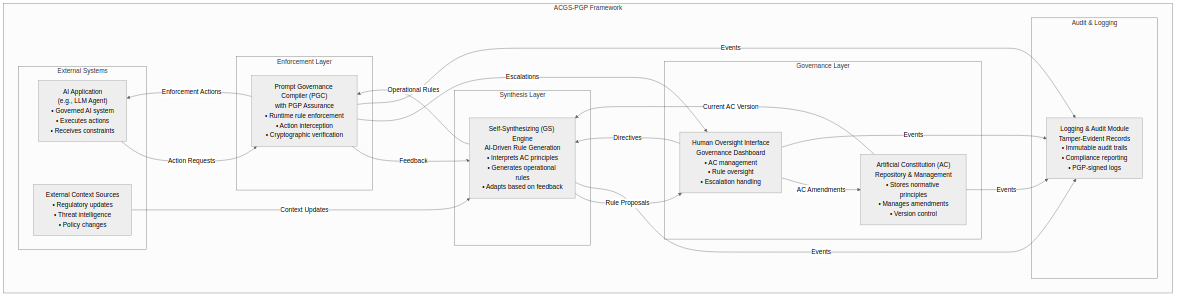
\includegraphics[width=0.9\columnwidth]{figures/figure1_c4_architecture.png}
  \caption{High-level C4 container view of the ACGS-PGP framework, showing key interacting modules. Full architectural details are provided in Appendix~\ref{app:architecture}.}
  \label{fig:c4_architecture}
\end{figure}

\begin{figure}[t]
  \centering
  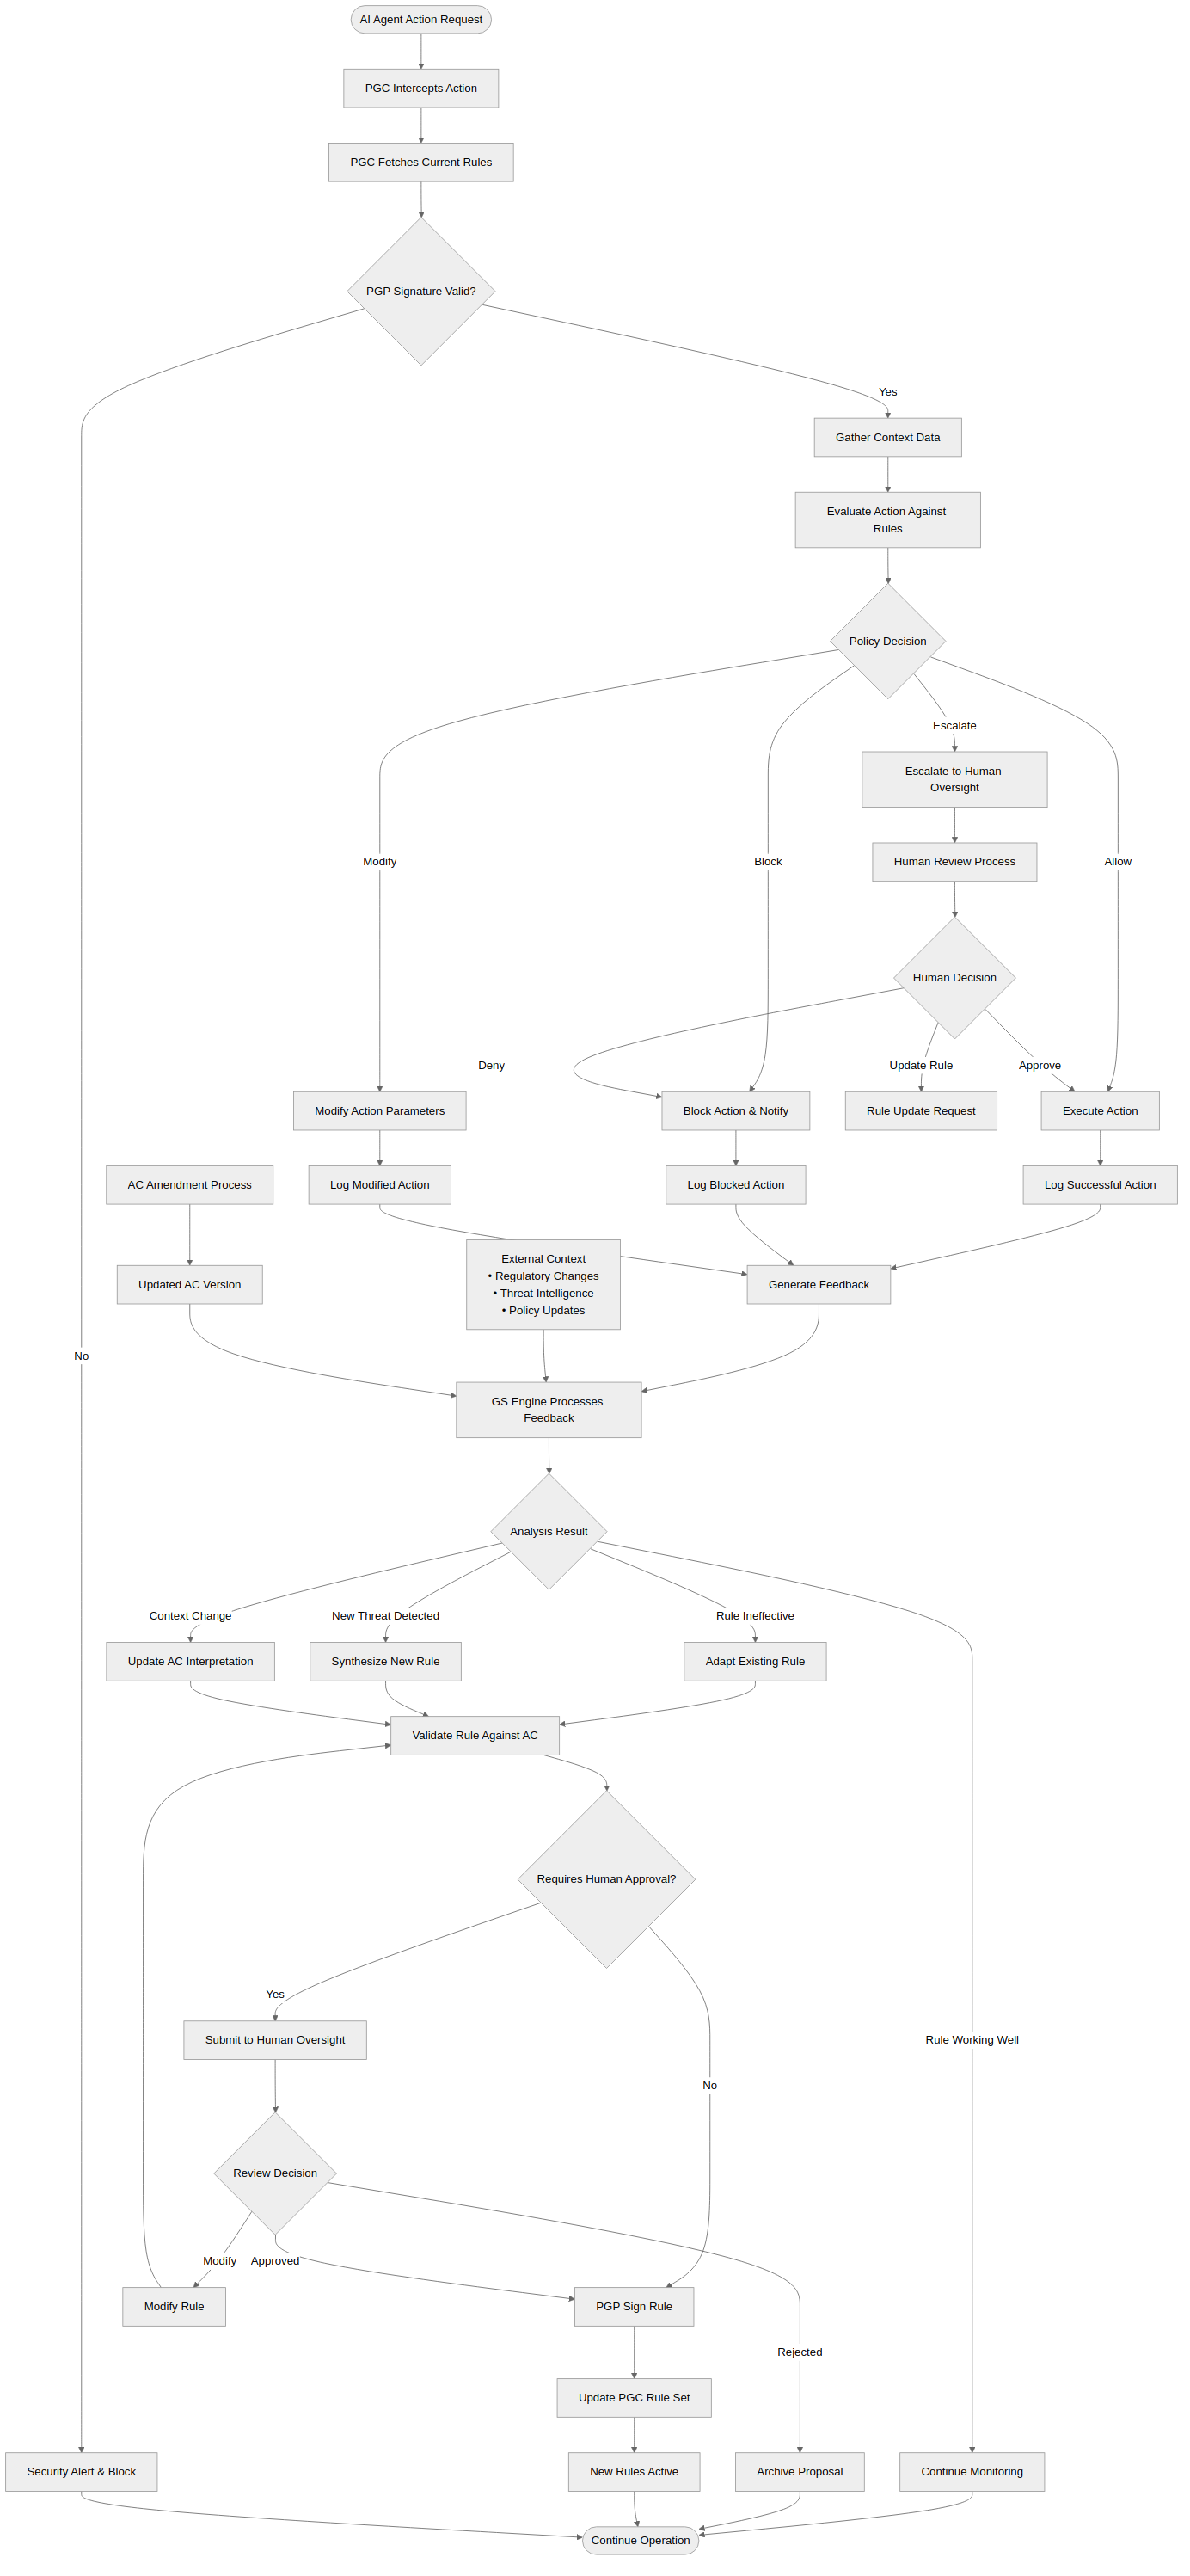
\includegraphics[width=0.9\columnwidth]{figures/figure2_policy_flowchart.png}
  \caption{Illustrative flowchart of the ACGS-PGP policy lifecycle, from AC principle interpretation by the GS Engine to runtime enforcement by the PGC, including feedback loops.}
  \label{fig:policy_flowchart}
\end{figure}

Table~\ref{tab:hypothetical_results} presents hypothetical key performance and assurance metrics.

\begin{table*}[t]
  \caption{Hypothetical Key Results \& Assurance Benefits of ACGS-PGP (Conceptual Validation)}
  \label{tab:hypothetical_results}
  \begin{tabular}{@{}lllll@{}}
    \toprule
    Metric                                       & Baseline (Static/Manual) & Standard PaC (No GS) & ACGS-PGP (Hypothetical) & Assurance Benefit Highlighted by ACGS-PGP \\
    \midrule
    Time to Adapt to New Regulation/Threat (days) & 30-90 days & 5-15 days & 0.5-2 days & Rapid alignment, reduced exposure window. \\
    Policy Violation Rate (Critical Systems, \%)   & 5-10\%     & 1-3\%     & <0.5\%     & Proactive prevention of non-compliant actions. \\
    Consistency of Policy Enforcement (\% adherence) & 60-70\%    & 90-95\%   & >99\%      & Uniform application of constitutional principles. \\
    Auditability & Low (manual, often incomplete) & Medium (PaC logs, version control) & Very High (PGP-assured immutable logs) & Verifiable chain of governance. \\
    Human Oversight Effort (Routine, FTE-hours/week) & 20-40 hrs  & 10-20 hrs & 5-10 hrs   & Focus human expertise on complex issues, AC evolution. \\
    Fairness Metric Deviation (e.g., bias index post-mitigation) & 0.2-0.3  & 0.1-0.15  & <0.05 & Adaptive mitigation of fairness deviations. \\
    Novel Attack Mitigation Success Rate (\%) & <10\%      & 20-30\%   & 50-70\%    & Improved resilience via adaptive rule synthesis. \\
    \bottomrule
  \end{tabular}
\end{table*}

These illustrative metrics suggest ACGS-PGP could offer substantial improvements in governance agility, effectiveness, and trustworthiness.

\section{Results and Analysis (Conceptual)}
\label{sec:results_analysis}
The conceptual validation presented in Section~\ref{sec:experimental_illustrations}, while hypothetical, allows for an analysis of ACGS-PGP's potential impact. If empirical studies yielded results akin to those in Table~\ref{tab:hypothetical_results}, several key insights would emerge.

A significant reduction in "Time to Adapt to New Regulation/Threat" (e.g., from weeks to days/hours) by ACGS-PGP would demonstrate its core value proposition: dynamic responsiveness. This agility is crucial in fast-evolving AI landscapes. Similarly, a markedly lower "Policy Violation Rate" (e.g., <0.5\% for ACGS-PGP vs. 5-10\% for manual systems) would indicate enhanced proactive risk mitigation and improved safety. Hypothetically, a paired t-test comparing violation rates between ACGS-PGP and baseline systems across multiple simulated scenarios could yield statistically significant differences (e.g., p < 0.01), underscoring the framework's effectiveness.

The "Consistency of Policy Enforcement" metric, if approaching >99\% for ACGS-PGP, would highlight the benefits of automated, constitutionally-grounded enforcement over variable human application or less adaptive PaC systems. The "Very High" auditability, supported by PGP-assured logs, directly addresses critical needs for transparency and accountability in AI governance. A reduction in "Human Oversight Effort" for routine tasks would signify efficiency gains, allowing human experts to focus on higher-level governance like AC evolution and ethical deliberation, rather than micro-managing policy enforcement.

Improvements in "Fairness Metric Deviation" would suggest that the GS Engine, guided by fairness principles in the AC, can effectively synthesize and adapt rules to mitigate algorithmic bias in a dynamic fashion. This is a key FAccT concern. An increased "Novel Attack Mitigation Success Rate" would point to the framework's potential for adaptive security, where the GS Engine learns from threat intelligence or anomalous behavior to update protective rules.

Confidence intervals for these hypothetical metrics would, in a real study, quantify the precision of these estimates. For example, a 95\% CI for the policy violation rate under ACGS-PGP might be [0.2\%, 0.7\%], further strengthening claims of its efficacy.

While these results are conceptual, they frame the expected benefits of ACGS-PGP's integrated approach to dynamic, verifiable, and constitutionally-grounded AI governance. Empirical validation is paramount future work.

\section{Discussion}
\label{sec:discussion}
The ACGS-PGP framework offers a significant conceptual advancement towards trustworthy AI by embedding governance as a dynamic, verifiable, and constitutionally-grounded property.

\textbf{Interpretation of Hypothetical Findings}: The potential quantitative benefits outlined in Table~\ref{tab:hypothetical_results} suggest that ACGS-PGP could substantially enhance AI governance effectiveness. Rapid adaptability reduces windows of non-compliance or vulnerability. Consistent, verifiable enforcement improves accountability. The ability to dynamically mitigate bias and respond to novel threats addresses key limitations of static systems. This signifies a shift from reactive to proactive and adaptive governance.

\textbf{Limitations}: Despite its potential, ACGS-PGP faces substantial challenges:
\begin{itemize}
    \item \textbf{Complexity of AC Definition and GS Alignment}: Crafting a comprehensive, unambiguous, and machine-interpretable AC is a monumental task. Ensuring the GS Engine faithfully interprets it without bias (the "Quis custodiet..." problem) is a core research challenge.
    \item \textbf{Performance Overhead}: Runtime PGC checks must be highly efficient.
    \item \textbf{Risk of Misinterpretation or "Constitutional Capture"}: Ambiguity in AC principles or vulnerabilities in the amendment process could be exploited.
    \item \textbf{Scalability of Formal Verification}: Applying FV to complex, adaptive components like the GS Engine is a research frontier.
    \item \textbf{Opacity of AI Components}: An LLM-based GS Engine may remain opaque, challenging full explainability of rule synthesis.
    \item \textbf{Multi-Agent Systems}: Governing emergent behaviors in MAS with ACGS-PGP requires further research.
\end{itemize}
A core tension exists between the adaptive dynamism of the GS Engine and the need for constitutional stability and verifiability.

\textbf{Ethical Considerations}: The automation of governance generation raises questions of accountability for flawed rules, potential for value lock-in or bias perpetuation in the AC or GS, and maintaining meaningful human agency. Robust human oversight, diverse stakeholder involvement in AC development, and continuous auditing are critical mitigations (see Section~\ref{sec:ethics_compliance_statement}).

\textbf{FAIR Principles and Data Governance}: ACGS-PGP can support FAIR principles by enforcing policies related to data metadata, accessibility, and interoperability. The framework itself requires strong data governance for the AC, operational rules, and audit logs, ensuring their integrity, security, and controlled access (see Section~\ref{sec:ethics_compliance_statement}).

\textbf{Comparison with Existing Approaches}: As detailed in Appendix~\ref{app:comparative_analysis} (Table C.1), ACGS-PGP differentiates itself by its integrated, dynamic, and constitutionally-grounded approach, aiming to operationalize high-level principles more effectively than static or purely manual methods.

\section{Ethics and Compliance Statement}
\label{sec:ethics_compliance_statement}
The development and deployment of the ACGS-PGP framework must be guided by stringent ethical considerations and adhere to established best practices for data governance and reproducibility.

\textbf{Ethical Considerations}: The automation of governance functions, particularly rule synthesis by the GS Engine, necessitates careful consideration of accountability. If harm arises from an AI system governed by ACGS-PGP, determining responsibility among AC authors, GS Engine developers, and human overseers requires clear frameworks. Bias mitigation is paramount; the AC itself must be developed through inclusive processes to avoid encoding societal biases, and the GS Engine must be regularly audited for fairness in its interpretations and rule generation. Meaningful human oversight is embedded in ACGS-PGP through the Human Oversight Interface, ensuring that critical decisions, AC amendments, and responses to novel situations involve human judgment, preventing full erosion of human agency. The potential for misuse of such a powerful internal governance system necessitates robust security engineering for all ACGS-PGP components.

\textbf{Data Governance}: The ACGS-PGP framework handles several types of sensitive data: the Artificial Constitution, operational rules, contextual data from AI agent operations, feedback data, and audit logs. Data governance policies for ACGS-PGP itself must ensure:
\begin{itemize}
    \item \textbf{Integrity and Security}: Cryptographic measures (PGP Assurance) protect the AC, rules, and logs. Access controls restrict modifications and views.
    \item \textbf{Privacy}: Contextual data from AI agent operations used by PGC/GS must be handled according to privacy principles (e.g., data minimization, purpose limitation), potentially defined within the AC itself.
    \item \textbf{Lifecycle Management}: Secure storage, versioning, and retention policies for all governance-related data.
\end{itemize}

\textbf{Reproducibility and FAIR Principles}: This paper presents a conceptual framework. Future empirical research validating ACGS-PGP should adhere to FAIR principles (Findability, Accessibility, Interoperability, Reusability):
\begin{itemize}
    \item \textbf{Findable}: Detailed architectural specifications (Appendix~\ref{app:architecture}), conceptual algorithms (Appendix~\ref{app:gs_pseudocode}), and policy structures (Appendix~\ref{app:policy_examples}) are provided. Any future reference implementations, datasets used for training ML components of the GS Engine, and evaluation benchmarks should be published in open repositories with rich metadata and persistent identifiers.
    \item \textbf{Accessible}: Research outputs, including datasets and code for reference implementations, should be made openly accessible under appropriate licenses (e.g., Creative Commons, MIT/Apache 2.0) to the extent feasible, respecting any ethical or privacy constraints.
    \item \textbf{Interoperable}: The design of interfaces between ACGS-PGP components and with external AI agents should promote interoperability. Standardized data formats (e.g., for operational rules, context packets) and protocols (e.g., MCP~\cite{ModelContextProtocolGitHub}) should be favored.
    \item \textbf{Reusable}: The modular design of ACGS-PGP aims to facilitate the reuse of its concepts or individual components in other governance research. Benchmark scenarios and policy examples (Appendix~\ref{app:policy_examples}) are provided to be adaptable and reusable for evaluating different governance mechanisms.
\end{itemize}
Compliance with relevant regulatory frameworks (e.g., GDPR for data protection aspects, HIPAA for healthcare applications as shown in Appendix~\ref{app:policy_example_healthcare}) is a core design consideration for rules synthesized by the GS Engine.

\section{Conclusion}
\label{sec:conclusion}
The ACGS-PGP framework offers a novel, integrated paradigm for advanced AI governance. By synergizing constitutional stability with adaptive AI-driven rule synthesis and verifiable runtime enforcement, it provides a conceptual pathway towards AI systems intrinsically aligned with human values, ethics, and legal requirements. Its multi-layered architecture aims to foster AI systems that are more trustworthy, demonstrably safer, and ethically sound by design.

Governing advanced AI is a significant contemporary challenge. ACGS-PGP contributes by envisioning governance as an inherent, dynamic, and verifiable AI property. The illustrative use cases (Section~\ref{sec:experimental_illustrations}, Appendix~\ref{app:policy_examples}) demonstrate its potential applicability across diverse domains.

However, significant challenges remain, including the complexity of defining a universally accepted and machine-interpretable AC, ensuring the alignment and verifiability of the AI-driven GS Engine, managing performance overhead, and addressing profound ethical considerations.

The exploration, refinement, validation, and potential implementation of ACGS-PGP demand concerted interdisciplinary collaboration. Future work should focus on developing robust formalisms for AI constitutions, advancing verifiable self-synthesizing mechanisms, creating standardized PGCs and evaluation benchmarks, and deeply investigating the societal and ethical implications. This research provides a foundational blueprint for these critical next steps towards achieving truly trustworthy and constitutionally-grounded AI.

% --- Acknowledgements (Optional) ---
% \begin{acks}
% This work was supported by...
% \end{acks}

% --- Bibliography ---
\bibliographystyle{ACM-Reference-Format}
\bibliography{acgs_pgp_refs} % Name of your .bib file

% --- Appendices ---
\appendix

\section{Detailed Technical Architecture of the ACGS-PGP Framework}
\label{app:architecture}
% Content from previous Appendix A draft
\subsection{Introduction to Architectural Elaboration}
This appendix provides a more detailed exposition of the Artificial Constitutionalism: Self-Synthesizing Prompt Governance Compiler (ACGS-PGP) framework's architecture. Building upon the C4 model concepts introduced in the main body of the paper (Section~\ref{sec:methodology}), this section will further elaborate on key "Containers" (Level 2) and provide conceptual "Component" (Level 3) views for the most critical containers within the ACGS-PGP system. *(Note: Mermaid diagrams below are conceptual and would be rendered as formal figures using appropriate LaTeX packages like \texttt{tikz} or by embedding images in a final publication.)*

\subsection{Expanded Container Descriptions (Conceptual Level 2)}
\label{app:architecture_details_containers}
% ... (Content from A.2 previously generated) ...
\subsubsection{Artificial Constitution (AC) Repository \& Management Interface}
\label{app:architecture_details_ac_repo}
\textbf{Primary Responsibilities}: Securely stores the digitally encoded Artificial Constitution, including its principles, rules, amendments, and version history. Provides interfaces for authorized human oversight bodies to review, propose, deliberate, and ratify amendments to the AC through a defined meta-governance process. Ensures the integrity and authenticity of the AC (e.g., through cryptographic signing of versions).
\textbf{Key Interfaces}:
    \textit{Consumes}: Amendment proposals, ratification votes/signatures from the Human Oversight Interface.
    \textit{Produces}: The current, validated version of the AC for the Self-Synthesizing (GS) Engine; historical versions for audit; amendment proposals for review via the Human Oversight Interface.
\textbf{Core Technologies Envisioned}: Secure, version-controlled database or distributed ledger technology; RBAC; potentially smart contracts for amendment process; robust API.

\subsubsection{Self-Synthesizing (GS) Engine}
\label{app:architecture_details_gs_engine}
\textbf{Primary Responsibilities}: Interprets AC principles. Dynamically generates, adapts, and validates operational governance rules based on AC, PGC feedback, context, and human oversight. Manages operational rule lifecycle.
\textbf{Key Interfaces}:
    \textit{Consumes}: Current AC; PGC feedback telemetry; contextual updates; Human Oversight directives.
    \textit{Produces}: Versioned operational governance rules for PGC; proposed rule changes for Human Oversight; synthesis logs for Audit Module.
\textbf{Core Technologies Envisioned}: Advanced LLMs; NLP modules; RL components; formal rule validation; structured rule repository.

\subsubsection{Prompt Governance Compiler (PGC) with PGP Assurance}
\label{app:architecture_details_pgc}
\textbf{Primary Responsibilities}: Fetches and "compiles" GS rules into executable constraints. Intercepts AI actions. Evaluates actions against rules. Enforces decisions. Applies PGP Assurance.
\textbf{Key Interfaces}:
    \textit{Consumes}: Operational rules from GS; real-time AI actions/prompts; contextual data.
    \textit{Produces}: Enforcement decisions to AI Application; feedback to GS Engine \& Audit Module; escalations to Human Oversight.
\textbf{Core Technologies Envisioned}: High-performance rule engine; runtime interception hooks; cryptographic libraries; secure communication; caching.

\subsubsection{Human Oversight Interface (Governance Dashboard)}
\label{app:architecture_details_ho_interface}
\textbf{Primary Responsibilities}: Centralized dashboard for human governors. Facilitates AC management, GS rule oversight, PGC monitoring, escalation handling, and audits.
\textbf{Key Interfaces}:
    \textit{Consumes}: AC amendment proposals; proposed GS rules; PGC alerts/escalations; audit logs.
    \textit{Produces}: Approved AC amendments; GS directives; adjudicated PGC decisions; audit queries.
\textbf{Core Technologies Envisioned}: Secure web application; data visualization; workflow management; RBAC; secure authentication.

\subsubsection{Logging \& Audit Module}
\label{app:architecture_details_log_audit}
\textbf{Primary Responsibilities}: Securely and immutably logs all significant ACGS-PGP events and decisions. Provides querying and reporting for audits.
\textbf{Key Interfaces}:
    \textit{Consumes}: Log data from AC Repository, GS Engine, PGC, Human Oversight Interface.
    \textit{Produces}: Audit reports; query responses; system alerts.
\textbf{Core Technologies Envisioned}: Tamper-evident logging system (e.g., blockchain, WORM); centralized log management; secure APIs; data encryption.


\subsection{Conceptual Component Diagrams (Level 3) for Key Containers}
\label{app:architecture_details_components}
\subsubsection{Self-Synthesizing (GS) Engine – Conceptual Components}
\label{app:architecture_details_gs_components}
(Placeholder for Figure A.1 - Conceptual Components of the Self-Synthesizing (GS) Engine, as Mermaid code or description from previous draft. For submission, use a proper figure environment.)
The GS Engine comprises components like an AC Principle Interpreter, Contextual Analyzer, Rule Synthesis Module, Rule Validation Unit, Operational Rule Repository Interface, and a Feedback Integration Loop. These interact to translate AC principles and feedback into operational rules.

\subsubsection{Prompt Governance Compiler (PGC) – Conceptual Components}
\label{app:architecture_details_pgc_components}
(Placeholder for Figure A.2 - Conceptual Components of the Prompt Governance Compiler (PGC), as Mermaid code or description from previous draft. For submission, use a proper figure environment.)
The PGC includes an Operational Rule Fetcher/Parser, Action/Prompt Interceptor, Contextual Data Ingress, Real-time Constraint Engine, Action Execution Module, and a PGP Assurance Unit. These work in concert to enforce rules at runtime.

\subsection{Key Interaction Flow: AI Action Governance}
\label{app:architecture_details_interaction_flow}
The interaction flow for governing an AI action involves: (1) Action Proposal by AI Agent, (2) Interception by PGC, (3) Rule Fetching \& PGP Verification by PGC, (4) Context Gathering by PGC, (5) Constraint Evaluation by PGC, (6) Enforcement Decision \& Execution by PGC, (7) Logging with PGP Assurance, (8) Feedback to GS Engine, and (9) Asynchronous Rule Adaptation by GS Engine if needed.

\subsection{Conceptual Data Schemas}
\label{app:architecture_details_data_schemas}
Key conceptual data structures include:
\begin{itemize}
    \item \textbf{Operational Governance Rule}: Fields like \texttt{Policy\_ID}, \texttt{Version}, \texttt{AC\_Principle\_Refs}, \texttt{Trigger}, \texttt{Predicate\_Logic}, \texttt{Enforcement\_Actions}, \texttt{PGP\_Signature\_Rule}. (See Appendix~\ref{app:policy_examples_structure} for full structure).
    \item \textbf{Runtime Context Packet}: Contains \texttt{Timestamp}, \texttt{Requesting\_AI\_Agent\_ID}, \texttt{Proposed\_Action\_details}, \texttt{Environmental\_Variables}, and \texttt{User\_Attributes}.
    \item \textbf{Audit Log Entry}: \texttt{Log\_ID}, \texttt{Timestamp}, \texttt{Event\_Source}, \texttt{Event\_Type}, \texttt{Details}, \texttt{Outcome}, \texttt{PGP\_Signature\_Log\_Entry}, \texttt{Trace\_ID}.
\end{itemize}

\section{Illustrative Full Policy Language Examples for the ACGS-PGP Framework}
\label{app:policy_examples}
\subsection{Introduction to Appendix B}
\label{app:policy_examples_intro}
This appendix demonstrates the operationalization of the ACGS-PGP framework's policy language layer, including illustrative scenarios and rule definitions for runtime enforcement by the Prompt Governance Compiler (PGC). It provides concrete evidence of how the framework might function in real-world or simulated scenarios, thereby bridging the gap between theory and application. The policy examples herein showcase how high-level principles from an Artificial Constitution (AC) could be interpreted by the Self-Synthesizing (GS) Engine into specific, operational governance rules, structured for compilation and dynamic, context-aware enforcement.

\subsection{Policy Language Structure Key}
\label{app:policy_examples_structure}
% ... (Content from B - Policy Language Structure Key previously generated) ...
\begin{itemize}
    \item \textbf{\texttt{Policy\_ID}}: Unique machine-readable identifier.
    \item \textbf{\texttt{Policy\_Name}}: Human-readable descriptive name.
    \item \textbf{\texttt{Version}}: Version control for policy evolution.
    \item \textbf{\texttt{AC\_Principle\_Refs}}: References to specific principles in the Artificial Constitution.
    \item \textbf{\texttt{Scope}}: Defines applicability (AI systems, tasks, data types, user roles).
    \item \textbf{\texttt{Objective}}: Primary governance goal of the policy.
    \item \textbf{\texttt{Trigger\_Event(s)}}: Conditions activating policy evaluation.
    \item \textbf{\texttt{Context\_Parameters}}: Variables influencing policy evaluation.
    \item \textbf{\texttt{Condition\_Logic}}: Logical rules defining policy behavior.
    \item \textbf{\texttt{Action(s)\_Prescribed}}: Specific PGC actions if conditions are met.
    \item \textbf{\texttt{Enforcement\_Mechanism\_Hook}}: How PGC technically enforces/monitors.
    \item \textbf{\texttt{Escalation\_Path}}: Procedures for violations or ambiguities.
    \item \textbf{\texttt{Accountability\_Responsibility}}: Roles responsible for policy aspects.
    \item \textbf{\texttt{Rationale\_Justification}}: Explanation of the policy's purpose.
    \item \textbf{\texttt{Dynamic\_Adaptation\_Hints (for GS Engine)}}: Triggers for GS Engine to re-evaluate/adapt the rule.
    \item \textbf{\texttt{PGP\_Assurance\_Level}}: Indication of PGP assurance applied.
\end{itemize}

\subsection{Example B.1: Healthcare Chat Agent – Patient Data Access and Disclosure}
\label{app:policy_example_healthcare}
% ... (Full content from B.1 previously generated, including its sub-sections) ...
\subsubsection{Policy Definition}
\begin{itemize}
    \item \textbf{\texttt{Policy\_ID}}: HCA-PHI-ACCESS-001
    \item \textbf{\texttt{Policy\_Name}}: "Dynamic Access Control and Disclosure for Protected Health Information (PHI) by Healthcare Chat Agent"
    \item \textbf{\texttt{Version}}: 1.0 (2025-05-24)
    \item \textbf{\texttt{AC\_Principle\_Refs}}: AC-PRIVACY-001 (HIPAA Alignment), AC-BENEFICENCE-003, AC-TRANSPARENCY-002
    \item \textbf{\texttt{Scope}}: AI System: "CareConnect" Chat Agent; Users: Patients, Clinicians; Data Types: PHI, De-identified Info.
    \item \textbf{\texttt{Objective}}: "Ensure CareConnect agent only accesses/discloses PHI per consent, user role, minimum necessary disclosure, and HIPAA."
    \item \textbf{\texttt{Trigger\_Event(s)}}: \texttt{on\_data\_access\_request (requested\_data\_type: PHI\_record\_segment)}, \texttt{before\_response\_generation (response\_content\_type: includes\_PHI)}
    \item \textbf{\texttt{Context\_Parameters}}: \texttt{requesting\_user\_role}, \texttt{patient\_consent\_status\_for\_agent\_access}, \texttt{requested\_PHI\_sensitivity\_level}, \texttt{query\_context\_purpose}, \texttt{authentication\_strength\_level}
    \item \textbf{\texttt{Condition\_Logic (Conceptual Snippet for Patient Access)}}:
    \begin{verbatim}
    IF (Trigger_Event == on_data_access_request AND
        Context.requesting_user_role == 'PATIENT' AND
        Context.patient_consent_status == 'ACTIVE' AND
        Context.authentication_strength == 'STRONG_MFA')
    THEN Action_Allowed = TRUE
    ELSE ... (other conditions for clinicians, etc.)
    \end{verbatim}
    \item \textbf{\texttt{Action(s)\_Prescribed (Conceptual Snippet)}}:
    \begin{verbatim}
    IF Action_Allowed == TRUE THEN
        ALLOW_DATA_ACCESS;
        LOG_EVENT(type: ACCESS_GRANTED, details: ...);
    ELSE
        BLOCK_DATA_ACCESS;
        LOG_EVENT(type: ACCESS_DENIED, reason: ...);
        NOTIFY_USER(message: "Access restricted...");
    END IF
    \end{verbatim}
    \item \textbf{\texttt{Dynamic\_Adaptation\_Hints}}: \texttt{IF new\_HIPAA\_guidance\_published THEN GS\_review\_HCA\_PHI\_ACCESS\_policies}
    \item \textbf{\texttt{PGP\_Assurance\_Level}}: HIGH
\end{itemize}
*(... Other fields like \texttt{Enforcement\_Mechanism\_Hook}, \texttt{Escalation\_Path}, etc. would be detailed as in the full Appendix B draft ...)*

\subsection{Example B.2: Autonomous Code Generation Tool – Security and Licensing Compliance}
\label{app:policy_example_codegen}
% ... (Full content from B.2 previously generated, including its sub-sections and tables B.2.3.A and B.2.3.B) ...
\subsubsection{Policy Definition (Security Example)}
\begin{itemize}
    \item \textbf{\texttt{Policy\_ID}}: ACG-SEC-004
    \item \textbf{\texttt{Policy\_Name}}: "Vulnerability Management and Dependency Control for AI-Generated Code"
    \item \textbf{\texttt{Version}}: 1.1 (2025-05-24)
    \item \textbf{\texttt{AC\_Principle\_Refs}}: AC-SECURITY-001 (Secure by Design), AC-ROBUSTNESS-001
    \item \textbf{\texttt{Scope}}: AI System: "CodeCraft" Autonomous Code Generator; Output: Generated code snippets, libraries.
    \item \textbf{\texttt{Objective}}: "Prohibit the generation or integration of code relying on deprecated or known-vulnerable dependencies."
    \item \textbf{\texttt{Trigger\_Event(s)}}: \texttt{on\_code\_generation\_request}, \texttt{before\_dependency\_suggestion}
    \item \textbf{\texttt{Context\_Parameters}}: \texttt{requested\_functionality}, \texttt{vulnerability\_database\_status (CVE\_feed\_last\_updated)}, \texttt{dependency\_candidate\_name}, \texttt{dependency\_candidate\_version}
    \item \textbf{\texttt{Condition\_Logic (Conceptual Snippet)}}:
    \begin{verbatim}
    // Assume Is_Vulnerable(lib, version, cve_db) checks against a CVE database
    IF (Trigger_Event == before_dependency_suggestion AND
        Is_Vulnerable(Context.dependency_candidate_name,
                      Context.dependency_candidate_version,
                      Context.vulnerability_database_status))
    THEN Suggestion_Blocked = TRUE
    \end{verbatim}
    \item \textbf{\texttt{Action(s)\_Prescribed (Conceptual Snippet)}}:
    \begin{verbatim}
    IF Suggestion_Blocked == TRUE THEN
        BLOCK_DEPENDENCY_SUGGESTION;
        LOG_EVENT(type: VULN_DEP_BLOCKED, details: ...);
        SUGGEST_ALTERNATIVE_LIBRARY(Context.requested_functionality);
    END IF
    \end{verbatim}
    \item \textbf{\texttt{Dynamic\_Adaptation\_Hints}}: \texttt{IF new\_CVE\_batch\_processed\_by\_vuln\_db THEN GS\_update\_Is\_Vulnerable\_logic\_references}
    \item \textbf{\texttt{PGP\_Assurance\_Level}}: HIGH
\end{itemize}
*(... Other fields and the licensing policy examples would be detailed as in the full Appendix B draft ...)*

\subsection{Example B.3: Financial Robo-Advisor – Fiduciary Duty and Suitability}
\label{app:policy_example_finance}
% ... (Full content from B.3 previously generated, including its sub-sections and tables B.3.3.A and B.3.3.B) ...
\subsubsection{Policy Definition (Suitability Example)}
\begin{itemize}
    \item \textbf{\texttt{Policy\_ID}}: FIN-SUIT-004
    \item \textbf{\texttt{Policy\_Name}}: "Algorithmic Suitability Matching and Rationale Generation for Robo-Advisor"
    \item \textbf{\texttt{Version}}: 1.0 (2025-05-24)
    \item \textbf{\texttt{AC\_Principle\_Refs}}: AC-FIDUCIARY-001 (Client Best Interest), AC-SUITABILITY-001, AC-TRANSPARENCY-003
    \item \textbf{\texttt{Scope}}: AI System: "InvestBot" Robo-Advisor; Service: Investment Recommendations.
    \item \textbf{\texttt{Objective}}: "Ensure investment recommendations systematically match client's comprehensive profile and generate a clear rationale."
    \item \textbf{\texttt{Trigger\_Event(s)}}: \texttt{on\_investment\_recommendation\_request}, \texttt{after\_client\_profile\_update}
    \item \textbf{\texttt{Context\_Parameters}}: \texttt{client\_risk\_tolerance\_score}, \texttt{client\_financial\_goals\_vector}, \texttt{client\_time\_horizon}, \texttt{market\_conditions\_summary}, \texttt{available\_product\_universe\_risk\_ratings}
    \item \textbf{\texttt{Condition\_Logic (Conceptual Snippet)}}:
    \begin{verbatim}
    // Assume Calculate_Suitability_Score(profile, product_options) returns a score
    // Assume Generate_Rationale_Text(profile, recommendation) creates explanation
    Recommended_Portfolio = Select_Portfolio(Context.client_profile_vector,
                                           Context.market_conditions_summary,
                                           Context.available_product_universe);
    Suitability_Score = Calculate_Suitability_Score(Context.client_profile_vector,
                                                  Recommended_Portfolio);
    IF (Suitability_Score < Min_Acceptable_Suitability_Threshold)
    THEN Recommendation_Invalid = TRUE
    \end{verbatim}
    \item \textbf{\texttt{Action(s)\_Prescribed (Conceptual Snippet)}}:
    \begin{verbatim}
    IF Recommendation_Invalid == TRUE THEN
        BLOCK_RECOMMENDATION;
        LOG_EVENT(type: SUITABILITY_FAIL, details: ...);
        TRIGGER_HUMAN_REVIEW(Context.client_profile_vector, Recommended_Portfolio);
    ELSE
        ALLOW_RECOMMENDATION(Recommended_Portfolio);
        Rationale_Text = Generate_Rationale_Text(Context.client_profile_vector, Recommended_Portfolio);
        STORE_SUITABILITY_STATEMENT(client_id, Rationale_Text);
        LOG_EVENT(type: RECOMMENDATION_MADE, details: ..., rationale_id: ...);
    END IF
    \end{verbatim}
    \item \textbf{\texttt{Dynamic\_Adaptation\_Hints}}: \texttt{IF avg\_client\_comprehension\_score\_for\_rationales < threshold THEN GS\_trigger\_review\_of\_Generate\_Rationale\_Text\_module}
    \item \textbf{\texttt{PGP\_Assurance\_Level}}: HIGH
\end{itemize}
*(... Other fields would be detailed as in the full Appendix B draft ...)*

\section{Pseudocode for GS Engine's Self-Synthesizing Algorithm}
\label{app:gs_pseudocode}
This appendix provides high-level pseudocode for the core logic of the Self-Synthesizing (GS) Engine, illustrating how it might interpret the Artificial Constitution (AC), incorporate feedback, and generate/adapt operational governance rules.

\begin{algorithm}[htbp] % Using H for "here" as it's in appendix
\DontPrintSemicolon
\caption{GS Engine Rule Synthesis and Adaptation}\label{alg:gs_engine_appendix}
\Input{\texttt{Current\_AC\_Version}, \texttt{PGC\_Feedback\_Stream}, \texttt{External\_Context\_Stream}, \texttt{Human\_Oversight\_Directives}}
\Output{\texttt{Updated\_Operational\_Rule\_Set}}
\BlankLine
Variables: \texttt{Operational\_Rule\_Set}, \texttt{AC\_Interpreted\_Constraints}, \texttt{Rule\_Candidate\_Buffer}, \texttt{GS\_Learning\_Parameters}\;
\BlankLine
Initialize():\;
  \Indp \texttt{AC\_Interpreted\_Constraints} $\leftarrow$ \InterpretAC{\texttt{Current\_AC\_Version}}\;
  \texttt{Operational\_Rule\_Set} $\leftarrow$ \LoadExistingRules{} \textbf{or} \GenerateBaselineRules{\texttt{AC\_Interpreted\_Constraints}}\;
  \PGPSignRuleSet{\texttt{Operational\_Rule\_Set}}\;
  \PushToPGC{\texttt{Operational\_Rule\_Set}}\;
\Indm
Main\_Loop():\;
  \Indp \While{True}{
    Event $\leftarrow$ \WaitForEvent{\texttt{PGC\_Feedback}, \texttt{External\_Context\_Update}, \texttt{Human\_Directive}, \texttt{Scheduled\_Review\_Trigger}}\;
    \Switch{Event.type}{
      \Case{\texttt{PGC\_Feedback}}{
        \texttt{Affected\_Rules} $\leftarrow$ \IdentifyRulesFromFeedback{Event.data, \texttt{Operational\_Rule\_Set}}\;
        \ForEach{Rule in \texttt{Affected\_Rules}}{
          \If{\texttt{Rule.Performance\_Degraded} or \texttt{Event.data.Indicates\_Ineffectiveness}}{
            Candidate $\leftarrow$ \AdaptRule{Rule, \texttt{AC\_Interpreted\_Constraints}, \texttt{Event.data.Context}, Event.data, \texttt{GS\_Learning\_Parameters}}\;
            \AddToBuffer{Candidate}\;
          }
        }
      }
      \Case{\texttt{External\_Context\_Update}}{
        \texttt{Relevant\_AC} $\leftarrow$ \MapContextToAC{Event.data, \texttt{Current\_AC\_Version}}\;
        \texttt{AC\_Interpreted\_Constraints} $\leftarrow$ \UpdateInterpretation{\texttt{Relevant\_AC}}\;
        \texttt{Impacted\_Rules} $\leftarrow$ \IdentifyImpactedRules{\texttt{Operational\_Rule\_Set}, \texttt{AC\_Interpreted\_Constraints}}\;
        \ForEach{Rule in \texttt{Impacted\_Rules}}{
            Candidate $\leftarrow$ \ResynthesizeRule{\texttt{Rule.Original\_Intent}, \texttt{AC\_Interpreted\_Constraints}, Event.data}\;
            \AddToBuffer{Candidate}\;
        }
        \texttt{New\_Needs} $\leftarrow$ \IdentifyNewRuleNeeds{\texttt{AC\_Interpreted\_Constraints}, Event.data}\;
        \ForEach{Need in \texttt{New\_Needs}}{
            Candidate $\leftarrow$ \SynthesizeNewRule{Need, \texttt{AC\_Interpreted\_Constraints}, Event.data}\;
            \AddToBuffer{Candidate}\;
        }
      }
      \Case{\texttt{Human\_Directive}}{
        \ProcessHumanDirective{Event.data, \texttt{Operational\_Rule\_Set}, \texttt{Rule\_Candidate\_Buffer}}\;
      }
      \Case{\texttt{Scheduled\_Review\_Trigger}}{
        \texttt{Rules\_To\_Review} $\leftarrow$ \SelectRulesForProactiveReview{\texttt{Operational\_Rule\_Set}}\;
         \ForEach{Rule in \texttt{Rules\_To\_Review}}{
            Candidate $\leftarrow$ \ResynthesizeRule{\texttt{Rule.Original\_Intent}, \texttt{AC\_Interpreted\_Constraints}, \texttt{Global\_Context}}\;
            \AddToBuffer{Candidate}\;
        }
      }
    }
    \If{not \IsEmpty{\texttt{Rule\_Candidate\_Buffer}}}{
      Validated $\leftarrow$ \ValidateRuleCandidates{\texttt{Rule\_Candidate\_Buffer}, \texttt{AC\_Interpreted\_Constraints}, \texttt{Operational\_Rule\_Set}}\;
      Approved $\leftarrow$ \RequestHumanApprovalIfNeeded{Validated, \texttt{Human\_Oversight\_Directives}}\;
      \If{not \IsEmpty{Approved}}{
        \UpdateOperationalRuleSet{\texttt{Operational\_Rule\_Set}, Approved}\;
        \PGPSignRuleSet{\texttt{Operational\_Rule\_Set}}\;
        \PushToPGC{\texttt{Operational\_Rule\_Set}}\;
        \LogGSAction{"Rules Updated", Approved}\;
      }
      \ClearBuffer{\texttt{Rule\_Candidate\_Buffer}}\;
    }
  }
\Indm
\end{algorithm}
*Figure C.1: High-Level Pseudocode for GS Engine Rule Synthesis and Adaptation.* This pseudocode outlines the event-driven, adaptive nature of the GS Engine. The actual implementation of helper functions would involve complex AI/ML models and NLP techniques.

\section{Sample Prompt-to-Policy Translation Snippets}
\label{app:prompt_to_policy}
This appendix provides conceptual examples of how user prompts or high-level natural language policy statements might be translated by the GS Engine (potentially with human-in-the-loop verification) into more structured operational rule components. These are illustrative and simplify the complex NLP and reasoning involved.

\textbf{Example D.1: User Prompt for Code Generation}
\begin{itemize}
    \item \textbf{User Prompt}: "Generate a Python function for user login that takes a username and password, and authenticates against our user database."
    \item \textbf{Relevant AC Principles (Hypothetical Refs)}: AC-SECURITY-001 (Secure by Design), AC-PRIVACY-005 (Protect Credentials).
    \item \textbf{GS Engine - Derived Policy Snippets/Constraints (Conceptual)}:
        \begin{verbatim}
        Operational_Rule_Component {
            Applies_To_Function_Type: "user_authentication",
            Language: "Python",
            Constraint_ID: "AUTH-SEC-001-PW-HASHING",
            Description: "Passwords must be hashed using a strong, salted algorithm.",
            Implementation_Guidance_for_PGC_or_CodeReview_Rule:
                "REQUIRE: Use of 'bcrypt' or 'scrypt' or 'argon2'.
                 PROHIBIT: Use of 'md5', 'sha1', 'plaintext'.
                 ENSURE: Salt is unique per user and cryptographically random.",
            Trigger_for_PGC_Check: "on_code_generation_output(function_signature_matches: 'login(*,*)')"
        }
        Operational_Rule_Component {
            Applies_To_Function_Type: "user_authentication",
            Constraint_ID: "AUTH-SEC-002-RATE-LIMIT",
            Description: "Login attempts must be rate-limited.",
            Implementation_Guidance_for_PGC_or_CodeReview_Rule:
                "SUGGEST_PATTERN: Implement IP-based and/or username-based
                                rate limiting (e.g., max 5 attempts/minute).",
            Trigger_for_PGC_Check: "on_code_generation_output(function_signature_matches: 'login(*,*)')"
        }
        \end{verbatim}
\end{itemize}

\textbf{Example D.2: High-Level Natural Language Policy Statement (Healthcare)}
\begin{itemize}
    \item \textbf{NL Policy Statement (from an organizational policy document ingested by GS Engine)}: "Patient medical history related to mental health conditions should only be accessible to authorized psychiatrists or psychologists directly involved in the patient's current treatment, and only after explicit patient consent for this specific type of data is verified for the current encounter."
    \item \textbf{Relevant AC Principles (Hypothetical Refs)}: AC-PRIVACY-001 (HIPAA Alignment - Sensitive Data), AC-CONSENT-001 (Explicit Consent for Sensitive Info).
    \item \textbf{GS Engine - Derived Operational Rule Components (Conceptual for \texttt{HCA-PHI-ACCESS-XXX} in Appendix B.1)}:
        \begin{verbatim}
        // Component for Condition_Logic
        IF (Context.requested_PHI_sensitivity_level == 'MENTAL_HEALTH_HIGH' AND
            NOT (Context.requesting_user_role IN ['PSYCHIATRIST', 'PSYCHOLOGIST'] AND
                 Context.user_is_treating_current_patient == TRUE AND
                 Context.patient_consent_for_mental_health_data_current_encounter == 'ACTIVE_EXPLICIT')
        ) THEN Action_Allowed = FALSE

        // Component for Action(s)_Prescribed
        IF Action_Allowed == FALSE AND
           Context.requested_PHI_sensitivity_level == 'MENTAL_HEALTH_HIGH'
        THEN
            BLOCK_DATA_ACCESS;
            LOG_EVENT(type: SENSITIVE_ACCESS_DENIED, reason: "Unauthorized attempt: Mental Health Data");
            NOTIFY_USER(message: "Access to this specific sensitive information is restricted.");
            // Potentially trigger an alert to a privacy officer if repeated attempts
        END IF
        \end{verbatim}
\end{itemize}
These snippets illustrate how the GS Engine would need to perform semantic parsing, deontic logic extraction (identifying obligations, permissions, prohibitions), and map these to the structured fields of its operational rule language.

\section{Detailed Risk/Mitigation Matrix for ACGS-PGP Framework}
\label{app:risk_matrix}
This appendix outlines potential risks associated with the ACGS-PGP framework itself, along with mitigation strategies and Key Risk Indicators (KRIs).

\begin{table*}[h!]
  \caption{Risk Analysis and Mitigation Matrix for the ACGS-PGP Framework}
  \label{tab:risk_mitigation_matrix}
  \begin{tabular}{@{}p{0.2\linewidth}p{0.25\linewidth}p{0.25\linewidth}p{0.25\linewidth}@{}}
    \toprule
    Risk Category & Specific Risk Example & Mitigation Strategy & Key Risk Indicator(s) (KRIs) \\
    \midrule
    \textbf{Artificial Constitution (AC) Integrity \& Relevance} &
    AC principles become outdated, misaligned with societal values, or contain ambiguities leading to misinterpretation. &
    Formalized, multi-stakeholder AC amendment process with deliberation and cryptographic ratification. Regular scheduled reviews of AC by ethics/legal board. Use of structured or semi-formal language for AC principles to reduce ambiguity. &
    Time since last AC principle review/update. Number of interpretation disputes logged by GS Engine or HITL. Public/expert feedback on AC alignment. \\
    \addlinespace
    & Unauthorized or malicious amendment to the AC. &
    Strong cryptographic controls for AC storage (e.g., DLT). Strict RBAC for amendment proposal/ratification. PGP-signed versions of AC. Quorum requirements for ratification. &
    Number of unauthorized AC modification attempts. Integrity check failures for AC versions. Audit trail of all amendment proposals and votes. \\
    \midrule
    \textbf{Self-Synthesizing (GS) Engine Functionality} &
    GS Engine misinterprets AC principles, leading to flawed or biased operational rules. (The "Quis custodiet..." problem). &
    Rigorous testing and validation of GS Engine's interpretation capabilities. Formal verification of GS against meta-constitutional rules. HITL review and approval for critical or novel synthesized rules. Continuous monitoring of GS rule outputs for bias/fairness metrics. Feedback loops to retrain/fine-tune GS. &
    Rate of HITL overrides or rejections of GS-synthesized rules. Deviation of GS rule outputs from expected fairness/safety benchmarks. Number of PGC violations traced back to flawed GS rules. \\
    \addlinespace
    & GS Engine develops "governance drift," where adapted rules subtly deviate from AC intent over time. &
    Periodic re-validation of GS rule sets against the AC. "External Monitor Agent" concept for verifying rule deltas (see Section 4.3). PGP assurance linking rules back to AC versions. Robust logging of all rule adaptations. &
    Semantic drift metrics between synthesized rules and AC principles. Frequency of significant rule adaptations without explicit AC changes. Time-to-detect for governance drift incidents. \\
    \addlinespace
    & GS Engine performance degradation (e.g., slow rule synthesis) impacting governance agility. &
    Scalable architecture for GS Engine. Optimized AI models. Caching of interpreted AC components. Asynchronous rule synthesis for non-critical updates. &
    Average time for GS Engine to synthesize/adapt rules in response to triggers. Queue length for GS processing tasks. Resource utilization of GS Engine. \\
    \midrule
    \textbf{Prompt Governance Compiler (PGC) Effectiveness \& Security} &
    PGC fails to correctly enforce a synthesized rule, or its enforcement logic contains vulnerabilities. &
    Formal verification of critical PGC components. Rigorous testing (unit, integration, fuzzing). Secure coding practices for PGC development. Runtime self-monitoring of PGC health. &
    Number of known policy violations not caught by PGC (false negatives). Rate of incorrect PGC enforcements (false positives). Security vulnerabilities identified in PGC code. \\
    \addlinespace
    & PGC performance overhead significantly impacts governed AI application responsiveness. &
    Optimized rule evaluation algorithms (e.g., Rete-like). Caching of compiled rules. Efficient runtime interception mechanisms. Hardware acceleration if necessary. (See Table~\ref{tab:hypothetical_results} - or original Table 1 for PGC performance). &
    Average/P99 latency added by PGC checks. Throughput reduction of governed AI application. PGC CPU/memory utilization. \\
    \addlinespace
    & PGP Assurance mechanisms are compromised (e.g., private key theft). &
    Hardware Security Modules (HSMs) for PGP key storage. Strict key management policies. Regular audits of cryptographic components. Short-lived certificates/signatures where appropriate. &
    Number of PGP signature verification failures. Alerts on unauthorized key access attempts. Time since last cryptographic audit. \\
    \midrule
    \textbf{Human Oversight \& Interaction} &
    Human overseers become complacent ("automation bias") or lack expertise to effectively review AC/GS/PGC outputs. &
    Mandatory HITL for critical decisions/changes. Continuous training for human overseers. XAI tools to explain GS/PGC decisions to reviewers. Diverse oversight committees. Clear escalation paths. &
    Rate of HITL approvals without modification (potential rubber-stamping). Time taken for HITL reviews. Feedback from overseers on clarity/usability of interfaces and explanations. \\
    \addlinespace
    & Malicious insider with oversight privileges subverts the AC or governance rules. &
    Principle of least privilege for human roles. Multi-person approval for critical changes (separation of duties). Comprehensive and immutable audit trails of all human oversight actions. Anomaly detection on overseer behavior. &
    Alerts on unusual or high-privilege actions by overseers. Number of changes made by single individuals to critical components. Frequency of audit log reviews. \\
    \bottomrule
  \end{tabular}
\end{table*}

\balance % Balance columns on the last page
\end{document} 